\documentclass[aspectratio=169]{beamer}

\usetheme{Madrid}

\definecolor{NavyTIPE}{RGB}{0,42,92}
\definecolor{CyanTIPE}{RGB}{0,160,200}
\definecolor{LightCyan}{RGB}{220,244,252}

\setbeamercolor{palette primary}   {bg=NavyTIPE, fg=white}
\setbeamercolor{palette secondary} {bg=CyanTIPE, fg=white}
\setbeamercolor{palette tertiary}  {bg=NavyTIPE, fg=white}
\setbeamercolor{palette quaternary}{bg=NavyTIPE, fg=white}
\setbeamercolor{structure}{fg=NavyTIPE}
\setbeamercolor{title}{fg=white, bg=NavyTIPE}
\setbeamercolor{frametitle}{fg=white, bg=NavyTIPE}
\setbeamercolor{block title}{bg=CyanTIPE, fg=white}
\setbeamercolor{block body}{bg=LightCyan, fg=black}
\setbeamercolor{alerted text}{fg=CyanTIPE}

\setbeamertemplate{bibliography item}{}

\usepackage[utf8]{inputenc}
\usepackage[T1]{fontenc}
\usepackage[french]{babel}
\usepackage{csquotes}

\usepackage{amsmath, amssymb}
\usepackage{graphicx}
\graphicspath{{imageIllustration/}}
\usepackage{hyperref}
\usepackage{array}
\usepackage{colortbl}

\usepackage{tikz}
\usetikzlibrary{arrows.meta, decorations.pathmorphing, decorations.markings,
decorations.pathreplacing, patterns, calc, positioning, shapes.geometric}

\usepackage{listings}
\definecolor{codegreen}{rgb}{0,0.6,0}
\definecolor{codegray}{rgb}{0.5,0.5,0.5}
\definecolor{codepurple}{rgb}{0.58,0,0.82}
\definecolor{backcolour}{rgb}{0.95,0.95,0.92}
\lstdefinestyle{mystyle}{
  backgroundcolor=\color{backcolour},
  commentstyle=\color{codegreen},
  keywordstyle=\color{NavyTIPE},
  numberstyle=\tiny\color{codegray},
  stringstyle=\color{codepurple},
  basicstyle=\ttfamily\tiny,
  breakatwhitespace=false,
  breaklines=true,
  captionpos=b,
  keepspaces=true,
  numbers=left,
  numbersep=5pt,
  showspaces=false,
  showstringspaces=false,
  showtabs=false,
  tabsize=2,
  literate={é}{{\'e}}1 {è}{{\`e}}1 {à}{{\`a}}1 {ç}{{\c{c}}}1 {œ}{{\oe}}1 {ù}{{\`u}}1 {À}{{\`A}}1 {É}{{\'E}}1 {ê}{{\^e}}1 {î}{{\^i}}1 {ô}{{\^o}}1 {û}{{\^u}}1 {â}{{\^a}}1
}
\lstset{style=mystyle}

\title[TIPE - Efficacité Propulsive]{%
  Influence de la flexibilité d'une hélice de drone\\
sur l'efficacité propulsive}
\subtitle{Simulation et Dispositif Expérimental}
\author{Merlin Claret}
\institute{PTSI — Lycée la Martinière Monplaisir, Lyon}
\date{23 Juin 2026}

\begin{document}

\begin{frame}[plain]
  \titlepage
\end{frame}

\begin{frame}{Plan}
  \tableofcontents
\end{frame}

\section{Contexte et lien au thème}

\begin{frame}{Contexte et enjeux}
  \begin{columns}
    \column{0.6\textwidth}
    \begin{itemize}
      \item Les drones ont de nombreuses applications nécessitant une \textbf{optimisation de l'autonomie}.
      \item En vol, les hélices subissent des charges aérodynamiques qui provoquent leur \alert{flexion}.
      \item Or, la rigidité dépend du matériau choisi. Une pale trop souple se déforme, ce qui modifie son angle d'attaque.
      \item \textbf{Question :} Cette déformation impacte-elle l'efficacité propulsive ?
    \end{itemize}

    \column{0.4\textwidth}
    \centering
    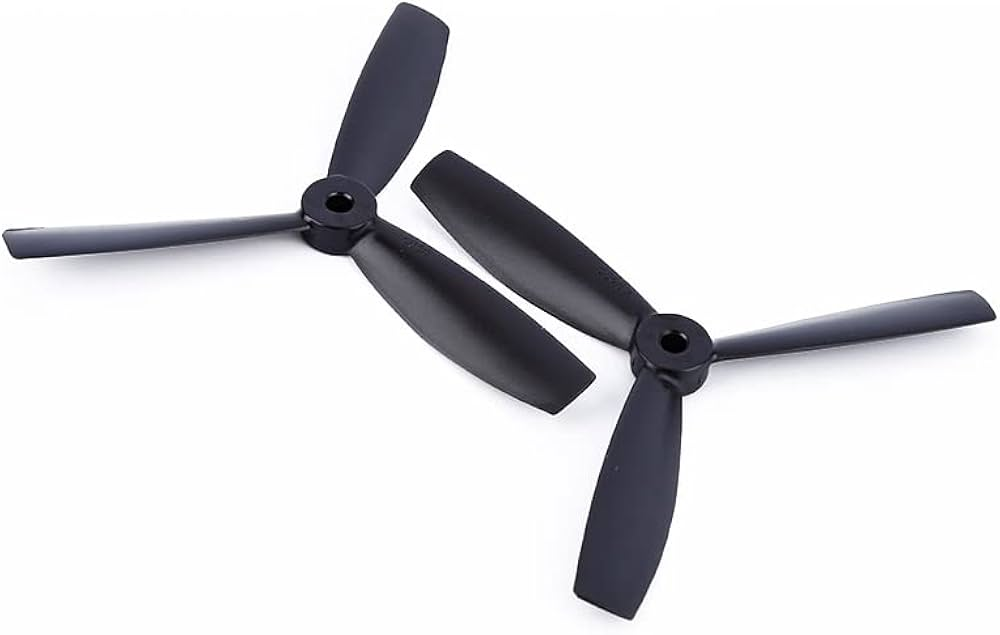
\includegraphics[width=\textwidth]{helice5pouce.jpg}
  \end{columns}
\end{frame}

\begin{frame}{Lien avec le thème de l'année}
  \begin{description}[\textbf{Optimisation}]
    \item[\textcolor{NavyTIPE}{Sobriété}]
      Limiter la masse de matière de l'hélice pour augmenter l'autonomie du drone.
    \item[\textcolor{NavyTIPE}{Efficacité}]
      Maximiser le rapport poussée générée / puissance consommée en tenant
      compte des déformations en vol.
    \item[\textcolor{NavyTIPE}{Optimisation}]
      Recherche du \alert{compromis de rigidité idéal} : ni trop souple
      (perte de poussée), ni trop rigide (surpoids).
  \end{description}
\end{frame}

\section{Évolution de la problématique}

\begin{frame}{Problématique initiale et obstacle}
  \begin{block}{Problématique d'origine}
    \textit{Quelle est l'influence du module d'Young d'une hélice de drone sur sa déformation en rotation et sur la perte d'efficacité propulsive ?}
  \end{block}

  \vspace{0.4cm}
  \textbf{Obstacles rencontrés :}
  \begin{itemize}
    \item Il est \alert{impossible d'imprimer en 3D} des hélices à causes des défauts de surface, et on ne peut pas pas tester différent matérieux facilement.
    \item Il est \alert{impossible d'acheter dans le commerce} des hélices de géométries identiques mais de rigidités différentes.
  \end{itemize}
\end{frame}

\begin{frame}{Nouvelle approche Semi-Empirique}
  \begin{itemize}
    \item \textbf{Solution possible:} Une approche semi-empirique sur des \alert{hélices commerciales} injectées (géométries parfaites).
      \begin{itemize}
        \item Sélection de deux hélices \textit{similaires} aux "extrêmes" de rigidité (ex: APC Nylon vs Gemfan Carbone).
        \item Mesure expérimentale de leur raideur propre $k$.
        \item Étude comparative basée sur l'\alert{écart de comportement à haut régime ($\Delta T$)} plutôt que sur la poussée absolue.
      \end{itemize}
  \end{itemize}

  \vspace{0.3cm}

  \begin{block}{Avantage de cette démarche}
    Cette méthode garantit d'isoler l'impact exclusif de la rigidité (\textbf{Résistance des Matériaux}) en éliminant le bruit des défauts d'impression.
  \end{block}
\end{frame}

\section{Simulation (Python)}

\begin{frame}{La simulation aéroélastique}
  \textbf{Modèle Python fonctionnel :} Couplage d'un modèle aérodynamique simplifié (\textit{Blade Element Theory}) et d'un \alert{modèle RDM} basé sur la théorie des poutres en torsion.

  \vspace{0.2cm}
  \begin{itemize}
    \item \textbf{Boucle de rétroaction simulée :}
      \begin{center}
        Torsion de la pale $\rightarrow$ Chute de l'angle d'incidence $\rightarrow$ Baisse de la poussée.
      \end{center}
      Le script itère jusqu'à trouver le point d'équilibre.
  \end{itemize}

  \vspace{0.2cm}
  \begin{alertblock}{Résultat de la simulation}
    À un régime réel de drone FPV (\textbf{25 000 tr/min}), le modèle prédit que la différence de flexibilité entre le Nylon et le Polycarbonate-Carbone génère un écart mesurable de l'ordre de \textbf{1 Newton ($\sim$100g force)}.
  \end{alertblock}
\end{frame}

\section{Conception du banc de test}

\begin{frame}{Le dispositif expérimental : Chariot pour éviter l'arc-boutement}
  \begin{columns}
    \column{0.6\textwidth}
    \small
    \textbf{Le Défi Mécanique :}
    \begin{itemize}
      \item Mesurer un écart de $100g$ nécessite l'absence totale de frottements parasites.
      \item Le décalage entre la poussée (en haut) et les axes (en bas) provoque un \alert{arc-boutement} (coincement).
    \end{itemize}

    \vspace{0.1cm}
    \textbf{La Solution CAO (SolidWorks) :}
    \begin{itemize}
      \item Structure rigide en "caisson" : plaques prises en sandwich par des \alert{tubes en aluminium et tiges filetées M4}.
      \item Entraxe des colonnes de 160 mm.
      \item Guidage allongé avec \textbf{4 brides LMK8UU} (2 sur la platine moteur, 2 en bas) coulissant sur des barres lisses de \textbf{8 mm} (fixées par des supports SHF8).
    \end{itemize}

    \column{0.4\textwidth}
    \centering
    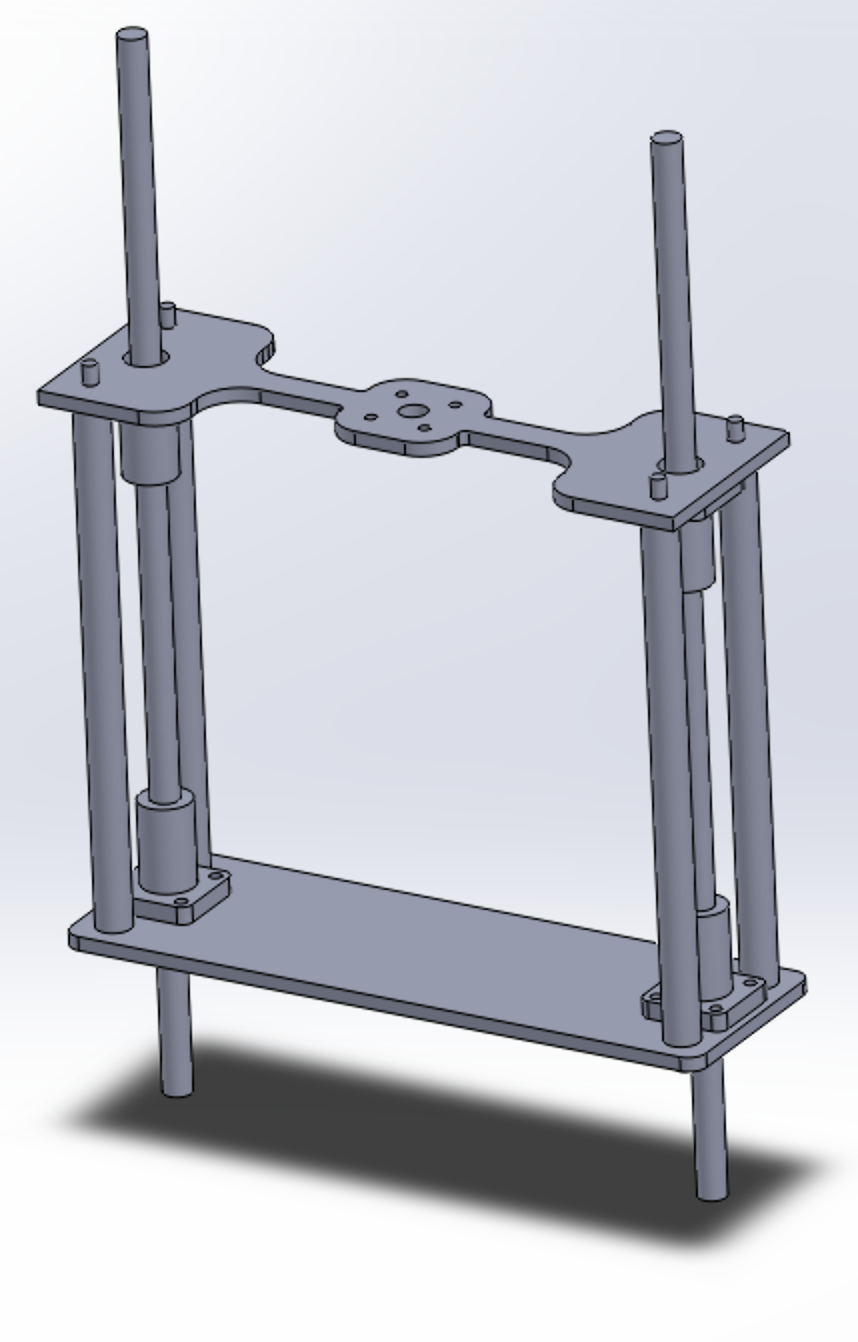
\includegraphics[width=\textwidth,height=0.65\textheight,keepaspectratio]{chariotAssembl.png}
  \end{columns}
\end{frame}

\section{Défis techniques}

\begin{frame}{Questions techniques en cours de résolution}
  \begin{columns}
    \column{0.5\textwidth}
    \textbf{1. Instrumentation de la poussée}
    \begin{itemize}
      \item \textit{Question :} Comment acquérir la poussée avec précision ?
      \item \textit{Pistes :} Balance de précision (simple) \textbf{vs} Cellule de charge avec Arduino et HX711 (complexe mais permet l'acquisition numérique en direct).
    \end{itemize}

    \vspace{0.3cm}
    \textbf{2. Matériaux et Usinage du chariot}
    \begin{itemize}
      \item \textit{Question :} Quel matériau pour les plaques du caisson ?
      \item \textit{Pistes :} Découpe laser sur \textbf{bois (3mm)} pour valider rapidement le prototype.
    \end{itemize}

    \column{0.5\textwidth}
    \textbf{3. Mesure statique de la raideur ($k$)}
    \begin{itemize}
      \item \textit{Question :} Comment obtenir une valeur expérimentale de $k$ pour le modèle ?
      \item \textit{Pistes :} Protocole de flexion statique avec masses et mesure de flèche.
    \end{itemize}

    \vspace{0.3cm}
    \begin{block}{Perspectives}
      Si le temps le permet, réintégrer l'\textbf{impression 3D} pour concevoir des hélices aux profils maîtrisés et tester les extrêmes de rigidité.
    \end{block}
  \end{columns}
\end{frame}

\section{Feuille de route}

\begin{frame}{Prochaines étapes (Feuille de route)}
  \begin{center}
    \renewcommand{\arraystretch}{1.5}
    \begin{tabular}{|>{\columncolor{NavyTIPE}\color{white}\bfseries}c|p{10cm}|}
      \hline
      Étape 1 & \textbf{Caractérisation statique :} Manipulation avec des masses pour mesurer la raideur réelle en flexion ($k$) des hélices. \\
      \hline
      \rowcolor{LightCyan}
      Étape 2 & \textbf{Validation RDM :} Injection des valeurs dans le script Python et confirmation de la déformation via \alert{SolidWorks Simulation}. \\
      \hline
      Étape 3 & \textbf{Fabrication :} Usinage des plaques, assemblage du chariot linéaire et des supports SHF8 sur le bâti. \\
      \hline
      \rowcolor{LightCyan}
      Étape 4 & \textbf{Campagne d'essais :} Acquisition des données (Poussée vs RPM) à haut régime pour valider le modèle. \\
      \hline
    \end{tabular}
  \end{center}
\end{frame}

\appendix
\section{Annexes}
\begin{frame}[allowframebreaks]{Annexe : Code Python (Aéroélasticité et RDM)}
  \lstinputlisting[language=Python]{../simulationStrategie1.py}
\end{frame}

\begin{frame}{Annexe : Résultats de la simulation}
  \centering
  \includegraphics[width=0.9\textwidth]{../resultatStrategie1.png}
\end{frame}

\end{document}
